\section{Introduction}
\label{sec:introduction}
Visual relocalization recovers the pose of a camera with respect to a previously mapped environment. A common solution is structure-based localization: image features are matched to 3D landmarks and the pose is recovered from the resulting 2D--3D correspondences~\cite{sarlin2019hloc,lepetit2009epnp}. The effectiveness of this formulation depends on a simple property of the map: a stored landmark should represent the image evidence that will be matched at query time, and its 3D position should be consistent with that evidence.

\begin{figure}[!t]
\centering
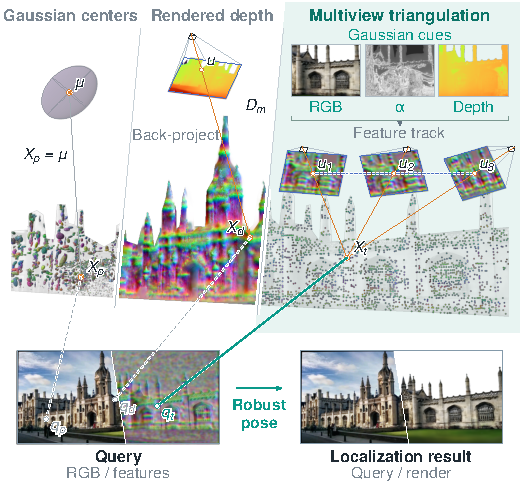
\includegraphics[width=\linewidth]{Fig1_geometry_to_localization.pdf}
\caption{From a Gaussian scene to a localization map. Gaussian centers and back-projected depth provide coordinate alternatives; our map triangulates multiview feature tracks. The lower panels show a query correspondence and alignment at the estimated Compact-map pose. Rendering visualizes the result and is not part of query localization.}
\label{fig:fig1}
\end{figure}


3D Gaussian Splatting (3DGS) has become a practical representation for reconstructing and rendering scenes~\cite{kerbl2023gaussian,huang2024_2dgs,guedon2025matcha}. This creates an appealing opportunity for localization: once a Gaussian scene is available, reference observations can be rendered from it instead of maintaining a separate localization map-building pipeline. The difficulty is that a rendering primitive is designed to contribute to image synthesis, whereas a localization landmark is used to explain a feature correspondence. These are related roles, but they do not require the same geometric representation. A Gaussian center is tied to a primitive rather than to a particular image feature, while a rendered depth value inherits the renderer's view-dependent depth assignment.

This distinction matters when a Gaussian scene is converted into an explicit localization map. The coordinate attached to a matched feature should be supported by the pixels that identify the same scene element across views. In other words, the rendering model should provide observations, while the observations themselves should determine the localization landmarks. This perspective keeps the geometric role of the Gaussian scene and that of the localization map separate without discarding the useful information provided by rendering.

\method{} follows this principle by constructing landmarks from multiview feature tracks on rendered reference views. Each track establishes which pixels correspond to one scene feature; calibrated rays from those pixels then determine a 3D position, and the same observations provide the landmark descriptor. Rendering is therefore used as an offline source of observations and geometric cues, not as the definition of the exported landmark. Figure~\ref{fig:fig1} summarizes this separation.

A second issue is that not every rendered observation is equally useful for correspondence construction. Local rendering artifacts, weak geometric support, and visually uninformative regions can produce detections that are distinctive but unreliable. We therefore filter observations before cross-view association, construct tracks using descriptor similarity together with epipolar geometry, and recover additional associations with rendered depth where the sparse camera graph leaves gaps. The resulting tracks are converted into landmarks by robust triangulation and view-balanced descriptor fusion. Finally, a localization-aware selector retains a compact subset by considering landmark quality, reference-view support, and the pose constraints supplied by the selected map.

The resulting system has a deliberately simple online interface. After offline construction, only landmark coordinates and descriptors are required. A query is matched directly to the compact 3D landmark map and localized with a robust pose solver, with no Gaussian rendering, image retrieval, or separate dense refinement at inference time. Thus the Gaussian scene remains the source of the map, while the deployed localization representation is an explicit, compact correspondence map.

The contributions are threefold:
\begin{enumerate}
\item \textit{Track-based landmark construction from Gaussian scenes.} We establish a correspondence-grounded conversion from a prebuilt Gaussian scene to an explicit localization map. Feature tracks, rather than Gaussian primitive identities, determine landmark geometry and appearance, with multiview triangulation providing the exported 3D coordinates.
\item \textit{Reliable observation and appearance construction.} We introduce a rendering-aware observation filtering procedure before association and a view-balanced multiview descriptor fusion scheme after tracking. Together they suppress unreliable rendered observations while preventing densely sampled viewpoints from dominating a landmark descriptor.
\item \textit{Localization-aware map selection.} We compact the reconstructed landmark bank by combining quality pruning, reference-view coverage completion, and pose-aware completion. The final map preserves complementary localization constraints while substantially reducing the deployed representation.
\end{enumerate}

We evaluate the resulting Compact map on \numScenes{} indoor and outdoor scenes and use the complete candidate bank, Full, to isolate the effect of selection. On Cambridge, Compact achieves $\numCompactTE\,cm/\numCompactRE^\circ$ average scene-median error with \numCompactStorage{}\,MB across five scenes. It retains 121,379 of 560,996 Full landmarks and reduces storage from \numFullStorage{}\,MB, while the Full reference reaches $\numCamTE\,cm/\numCamRE^\circ$. Additional experiments evaluate coordinate sources, observation filtering and descriptor fusion, alternative selection strategies, seven Gaussian model configurations, and the optional use of original mapping images.